\section{Event Selections} \label{section:higgs_selections}
For the purpose of reconstruction of physics objects of interest, CMS utilizes a Particle Flow Algorithm~\cite{CMS-PAS-PFT-10-002}, which aims to identify individual final state particles: photons, electrons, various hadrons, muons, etc. The main idea behind this algorithm is to use information not just from a particular subsystem (Muon, HCAL, ECAL, Tracker), but to combine and cross-reference features from various subdetectors: hits in the Tracker with Muon Stations, or clusters of energy depositions in ECAL, etc. In other words, this is an example of a sophisticated clusterization technique aimed to improve the resolution of energy and momentum reconstruction. For more information on the internals of the Particle Flow Algorithm, in particular in application to the CMS detector, consult the references \cite{Beaudette:2014cea}, \cite{Sirunyan:2017ulk}.

%For the purpose of our search, given the potential final states, the most important physics objects to be used are muons and jets. On top,
\subsection{HLT Selections}
The search requires one of the following Single Isolated Muon Triggers to fire per event:
\begin{itemize}
  \item HLT\_IsoMu24
  \item HLT\_IsoTkMu24
\end{itemize}
The choice of the threshold is driven by the requirement of the availability of the trigger for the whole period of datataking with the lowest p$_t$ threshold. These triggers require the event to have at least one isolated muon candidate with p$_t$ above 24 GeV, with no explicit restriction on its pseudorapidity.

\subsection{Primary Vertex Selections}
Primary Vertex is the measured position, together with the associated uncertainty, of a vertex that corresponds to the proton-proton interaction. The identification and reconstruction of all primary vertices per a given event is done by first, selecting all the tracks that seem to originate from a common vertex, and then further performing a regression to actually identify the position of that vertex. One of the top requirements on selecting a proton-proton collision event is the presence of at least one valid Primary Vertex with the following conditions:
\begin{itemize}
  \item $ndf \ge 4$ - number of tracks originating from this PV is greater than four
  \item $\rho < 2$ cm and $|Z| < 24$ cm - displacement along either Z-axis or in the transverse plan should be minimal w.r.t. the Interaction Point, defined as the origin.
\end{itemize}

\subsection{Muon Selections}
The muon candidates are reconstructed using the Particle Flow Algorithm by matching compatible track segments from the inner silicon tracker and the muon detectors~\cite{Chatrchyan:2012xi}. In our analysis, muons are required to be  within the pseudorapidity range $|\eta|<2.4$ and with a minimum transverse momentum $p_{t}>10$ GeV. Furthermore, muons are constrained to have $\Delta \beta$-corrected relative isolation, defined in Equation~\ref{eq:higgs_selections_isolation}, of $I_{rel}^{PF}<0.25$. In the definition of the isolation variable $p_{T}^{ch}$ is the charged hadron transverse sum of individual momenta, $E_{T}^{\gamma}$ is the photon transverse energy sum, and $E_{T}^{nh}$ is the neutral hadron transverse energy sum. The term $p_{T}^{chPU}$ is the estimated transverse momentum of charged particles from pileup in the $\Delta R < 0.4$ cone (defined in Equation~\ref{eq:higgs_selections_deltar}) and the factor of 0.5 is used to estimate the neutral pileup from the charged component.
\begin{center}
   \begin{equation}
      \label{eq:higgs_selections_deltar}
      {\Delta R} = {\sqrt{\Delta\eta^{2}+\Delta\phi^{2}}}
   \end{equation}
\end{center}
\begin{center}
   \begin{equation}
      \label{eq:higgs_selections_isolation}
      {I_{rel}^{PF}} = {(p_{T}^{ch}+max(0,E_{T}^{\gamma}+E_{T}^{nh}-0.5*p_{T}^{chPU}))/p_{t}}
   \end{equation}
\end{center}

Additionally, only ``Medium Id'' muons are selected - centrally provided and recommended by the CMS Physics Object Group~\cite{CMSMuonPOG,CMSMuonId}. As it was mentioned previously, muons are reconstructed using clusters of hits from various subsystems (Tracker and Muon Stations); in other words a physics object muon is defined to be a composite cluster of combined hits from the Tracker and Muon Systems. It is important to understand the difference between the actual physical particles, which are muons, and the definition of a reconstructed muon! Moreover, when extracting the momentum of a muon, a regression procedure is performed, a fit for instance, from which it is possible to extract the goodness of fit or some other quality metric, using which one can judge the quality of the reconstructed candidate. Finally, ``Muon Id'' is a set of criteria that defines a muon candidate of certain quality and allows to discriminate candidates based on this feature.

\subsection{Muon Corrections}
Given a very narrow theoretical width of the Higgs Boson, $4.2$ MeV, the Higgs peak is dominated by the detector resolution which is on the order of several GeV. Therefore, to increase the sensitivity of the search, it is crucial to have the best possible dimuon mass resolution, both in data and Monte Carlo. Moreover, as it is going to be described further in the Section~\ref{section:higgs_signalmodel}, it is necessary to correct for possible dimuon mass scale shifts.

There are two different sets of Muon corrections derived centrally within the CMS collaboration that are to be used separately: Rochester~\cite{CMSRochesterCorrections} and Kalman~\cite{CMSKalmanCorrections}. Both allow to correct the scale and smear the resolution. For the validation purposes, both sets of corrections are applied and the effects on Z scale and resolution are evaluated. In Figures~\ref{fig:higgs_selections_zscale} and ~\ref{fig:higgs_selections_zresolution} comparisons of uncorrected versus corrected results are shown for the scale and resolution, respectively. Both the Rochester and Kalman muon corrections successfully align Data with MC in terms of the Z peak. The impact of the two sets of corrections on the expected limits was evaluated and compared. It was found that the choice of one or another produces negligible difference for the expected limit, therefore final selections use the Rochester corrections.
\begin{figure}[p]
  \centering
  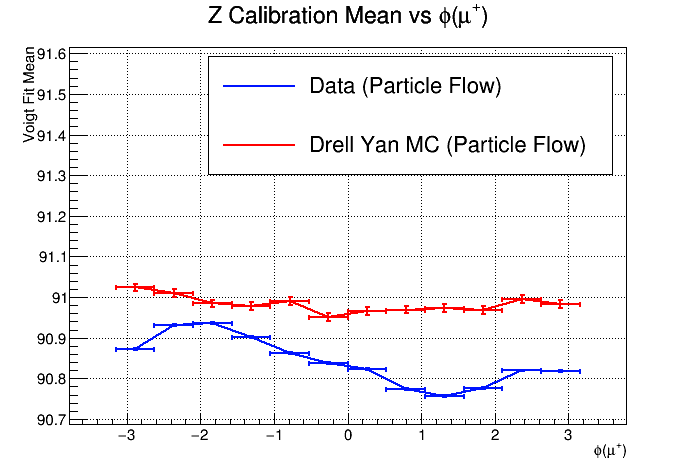
\includegraphics[width=0.32\linewidth]{figures/muon_calib/zcal_pf_mc-data_mean_phi_plus.png}
  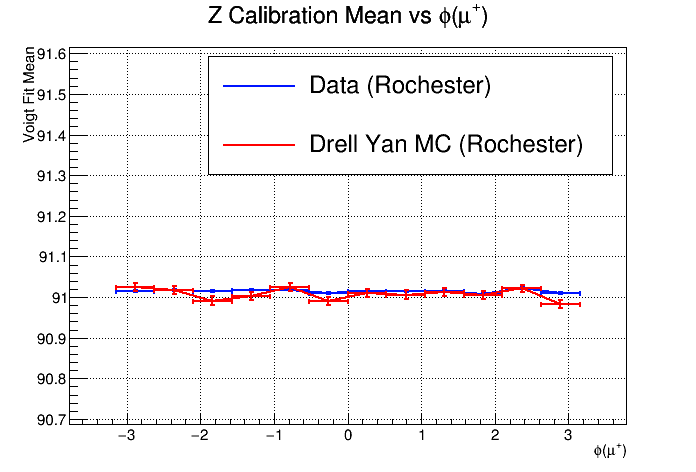
\includegraphics[width=0.32\linewidth]{figures/muon_calib/zcal_roch_mc-data_mean_phi_plus.png}
  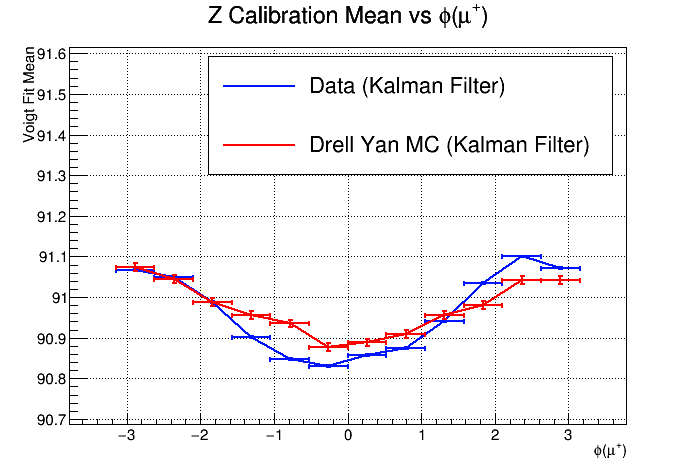
\includegraphics[width=0.32\linewidth]{figures/muon_calib/zcal_kamu_mc-data_mean_phi_plus.png}\\
  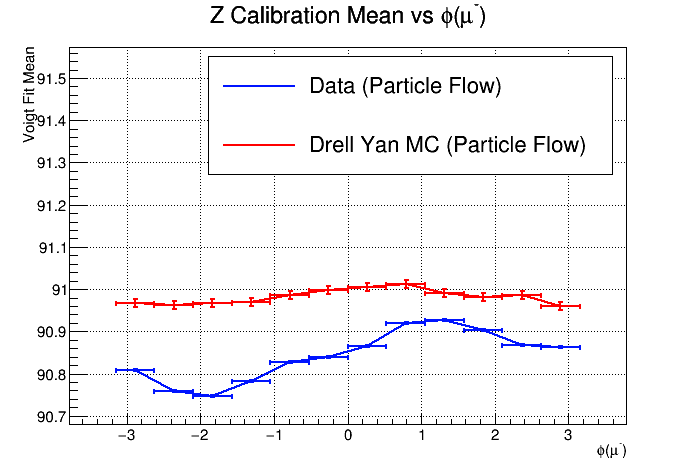
\includegraphics[width=0.32\linewidth]{figures/muon_calib/zcal_pf_mc-data_mean_phi_minus.png}
  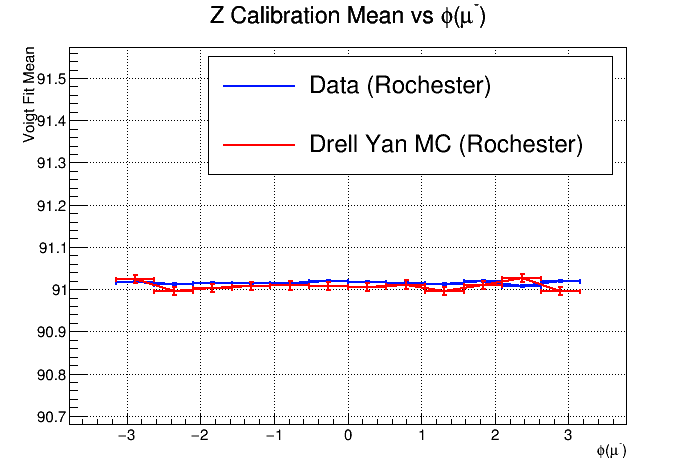
\includegraphics[width=0.32\linewidth]{figures/muon_calib/zcal_roch_mc-data_mean_phi_minus.png}
  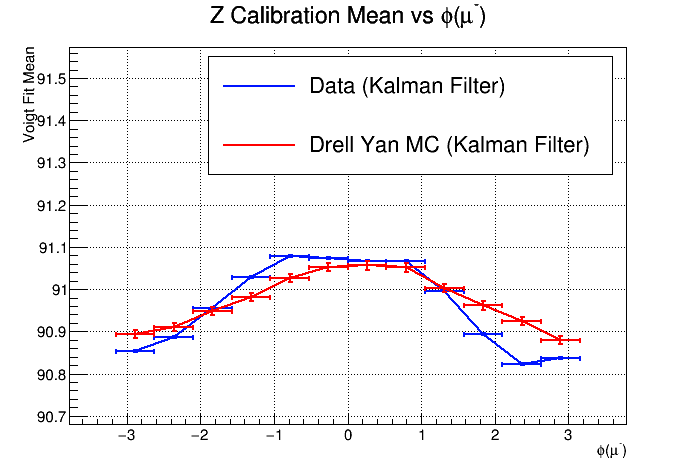
\includegraphics[width=0.32\linewidth]{figures/muon_calib/zcal_kamu_mc-data_mean_phi_minus.png}
  \caption{Comparing Uncorrected (left), Rochester (center) and Kalman (right) Corrections effects on the Z Scale (mass). Top (Bottom) three plots correspond to the Z mean vs phi of the first (second) muon from the candidate pair.}
  \label{fig:higgs_selections_zscale}
\end{figure}
\begin{figure}[p]
  \centering
  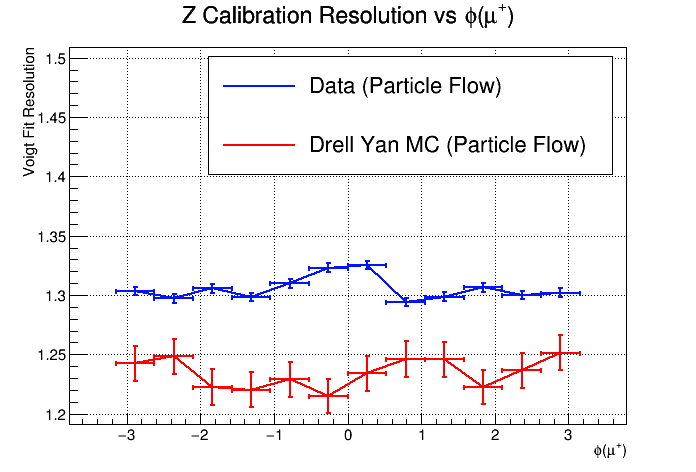
\includegraphics[width=0.32\linewidth]{figures/muon_calib/zcal_pf_mc-data_res_phi_plus.png}
  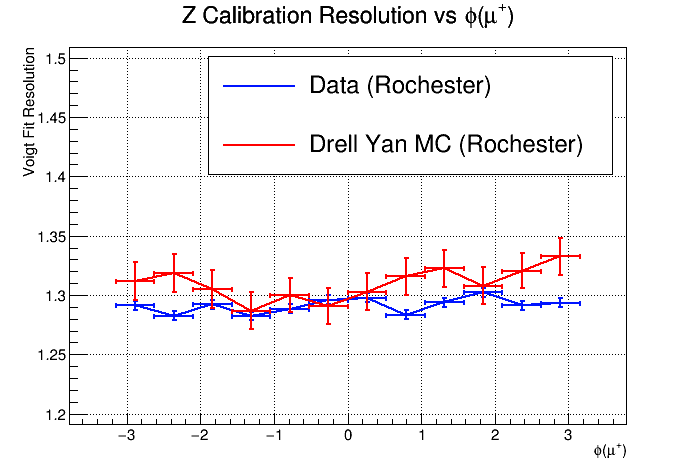
\includegraphics[width=0.32\linewidth]{figures/muon_calib/zcal_roch_mc-data_res_phi_plus.png}
  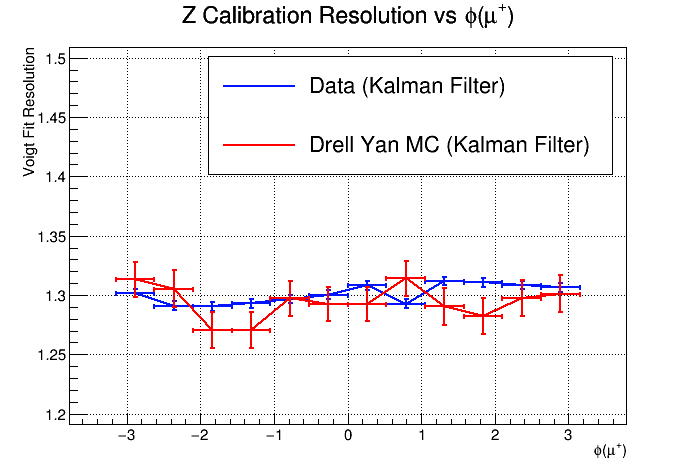
\includegraphics[width=0.32\linewidth]{figures/muon_calib/zcal_kamu_mc-data_res_phi_plus.png}\\
  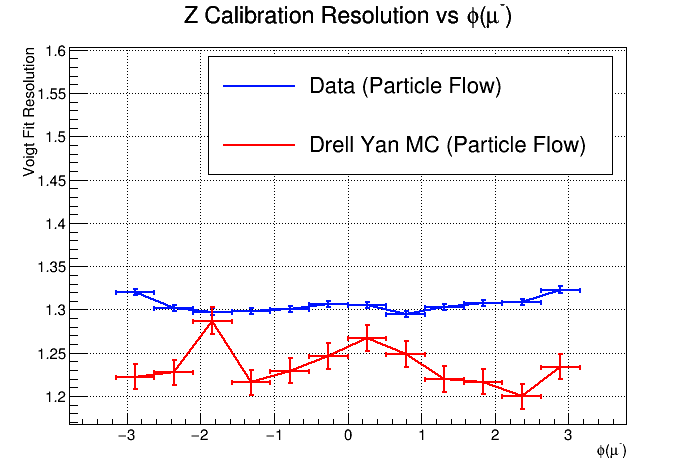
\includegraphics[width=0.32\linewidth]{figures/muon_calib/zcal_pf_mc-data_res_phi_minus.png}
  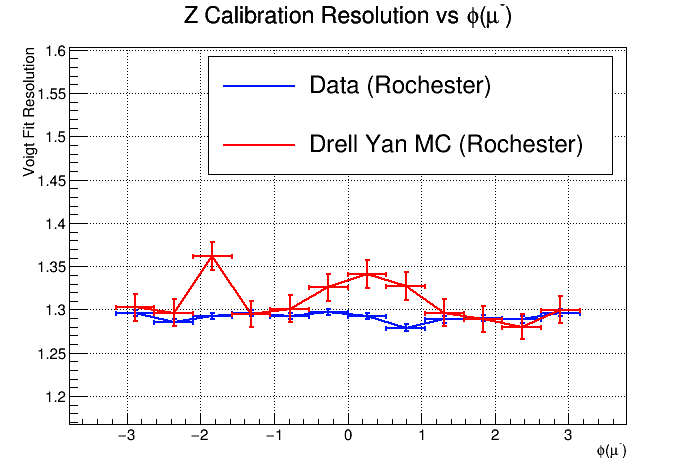
\includegraphics[width=0.32\linewidth]{figures/muon_calib/zcal_roch_mc-data_res_phi_minus.png}
  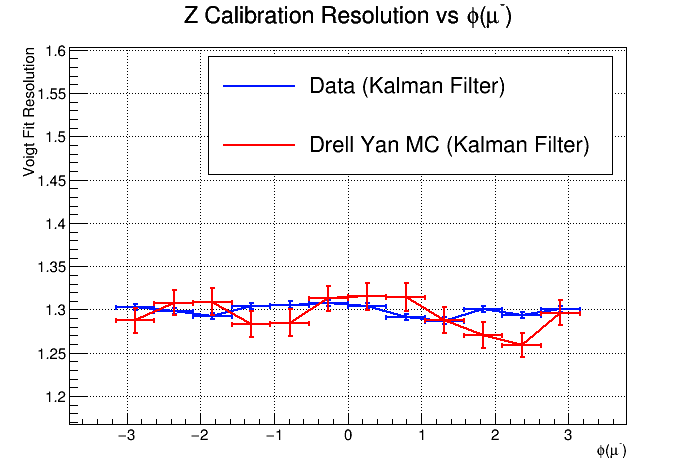
\includegraphics[width=0.32\linewidth]{figures/muon_calib/zcal_kamu_mc-data_res_phi_minus.png}
  \caption{Comparing Uncorrected (left), Rochester (center) and Kalman (right) Corrections effects on the Z Resolution (width). Top (Bottom) three plots correspond to the Z width vs phi of the first (second) muon from the candidate pair.}
  \label{fig:higgs_selections_zresolution}
\end{figure}

\subsection{Jet Selections}
Jets are reconstructed from PF candidates with the anti-$\kappa_{T}$ algorithm~\cite{Cacciari:2008gp} with a distance parameter of 0.4 after rejecting the charged hadrons that are associated to pileup primary vertices. Jets are ``cleaned'' against muons - jets overlapping with the selected PF muons, $\Delta R < 0.4$, are not considered further in the analysis. The selected jets with a minimum p$_t$ of 30 GeV and a maximum $|\eta|$ of 4.7 are corrected in energy in order to account for non-uniform detector response.

The PF jets are further required to fulfill the jet identification criteria.
Candidates with $|\eta|$ less than 2.7 are required to contain at
least one charged PF candidate and have a non-zero charged energy fraction,
and a charged electromagnetic energy fraction less than 0.99. The
neutral and photon energy fractions must be less than 0.99. Jets in
the region $2.7<|\eta|<3.0$ are required to have a neutral electromagnetic
fraction of greater than 0.01 and neutral hadron fraction less than
0.98 while jets with pseudorapidity above 3.0 are required to have more
than ten neutral particles and a neutral electromagnetic energy fraction
less than 0.9.

For reconstructed jets with $|\eta| < 2.4$, the combined secondary vertex (CSV) b-tagging algorithm \cite{Chatrchyan:2012jua} is used to discriminate against the $t\bar{t}$ background process. The CSV medium operating point is chosen as the baseline for the search analysis and corresponds to a b-tagging efficiency of $60-65\%$ while the misidentification rate for light quarks such as $u$, $d$, $s$, and gluon jets is at the order of 1\%.

\subsection{Selections Summary}
Cuts and selections can be summarized for the search as follows:
\begin{itemize}
  \item At least 1 Primary Vertex passing the PV Selections
  \item At least 1 of the HLT Paths fired
  \item At least 2 opposite sign muons which pass Muon Selections. If more than 1 pair - choose the 2 candidates with the highest \pt. That is the Higgs Candidate.
  \item At least 1 muon from the Higgs Candidate pair with $p_t > 26$ GeV and is matched to the HLT Path that fires the event with $\Delta R < 0.1$.
  \item Filter out the jets that do not pass the Jet Selections, but do not require a certain number of them at this stage.
\end{itemize}

\subsection{Validation}
After applying all of the specified selections, a set of events is selected that is going to be further used in order to maximize the sensitivity of the search. However, before proceeding to the next section, validation of basic kinematic distributions needs to be considered for the inclusive set of events.

First, in Figure~\ref{fig:higgs_selections_inclusivemassnocorr}, the inclusive dimuon mass distribution is presented without any muon momentum corrections applied. Notice the presence of a discrepancy near the Z mass ($\approx 91$ GeV) peak. It is the result of a discrepancy in both the mass scale and resolution.
\begin{figure}[htbp]
  \centering
  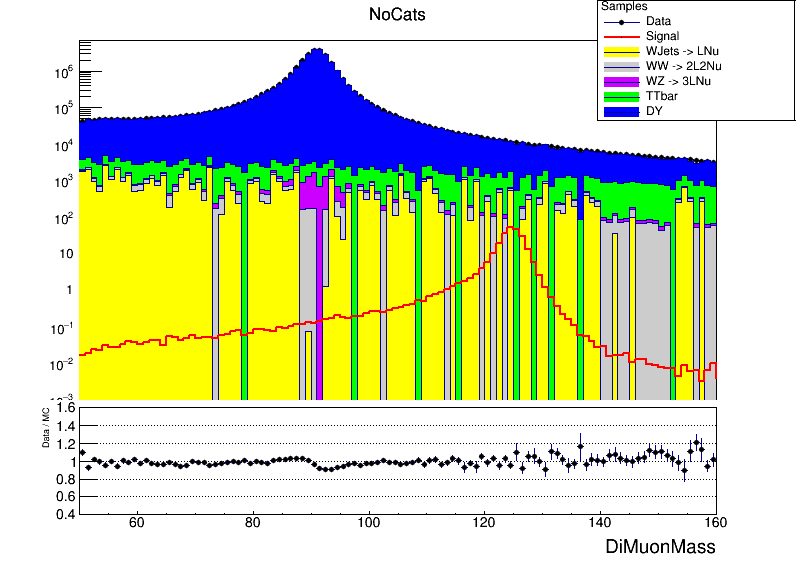
\includegraphics[width=0.5\linewidth]{figures/ch_higgs/distributions/baseline_nocorrections/distribution__NoCats__DiMuonMass__logY.png}
  \caption{Inclusive Dimuon Mass Distributions without any Muon Corrections. Comparison of data (black points) and simulated backgrounds (stacked). 125 GeV Higgs Boson signal is shown as a red solid line. The discrepancy around the Z mass peak of 91 GeV is circled in red.}
  \label{fig:higgs_selections_inclusivemassnocorr}
\end{figure}

 Second, in Figure~\ref{fig:higgs_selections_inclusivekinematic}, distributions of various kinematic variables after passing the selections are presented. Overall, data is well modeled; however, there are some deviations in particular for the p$_t$ of the dimuon system. Up to 40\% discrepancy is observed; however, only for a small region around 50 GeV. For the muon p$_t$, the observed deviation happens only for the transverse momentum values below the 26 GeV threshold that is being used for the muon matching the HLT. It is crucial to point out that although there are deviations in the modeling of some of the kinematic distributions, the modeling of the dimuon mass distribution shows very good agreement between the data and the simulated backgrounds.
  \begin{figure}[htbp]
    \centering
    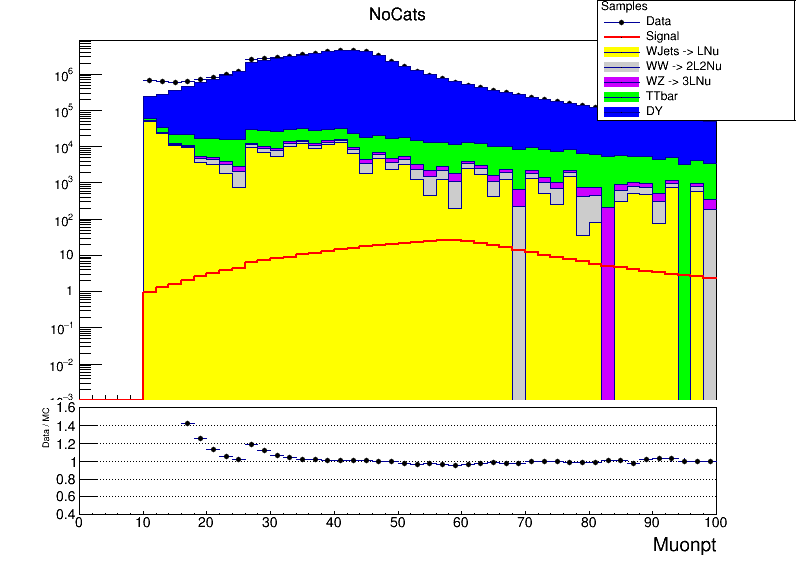
\includegraphics[width=0.45\linewidth]{figures/ch_higgs/distributions/baseline_kalman/distribution__NoCats__Muonpt__logY.png}
    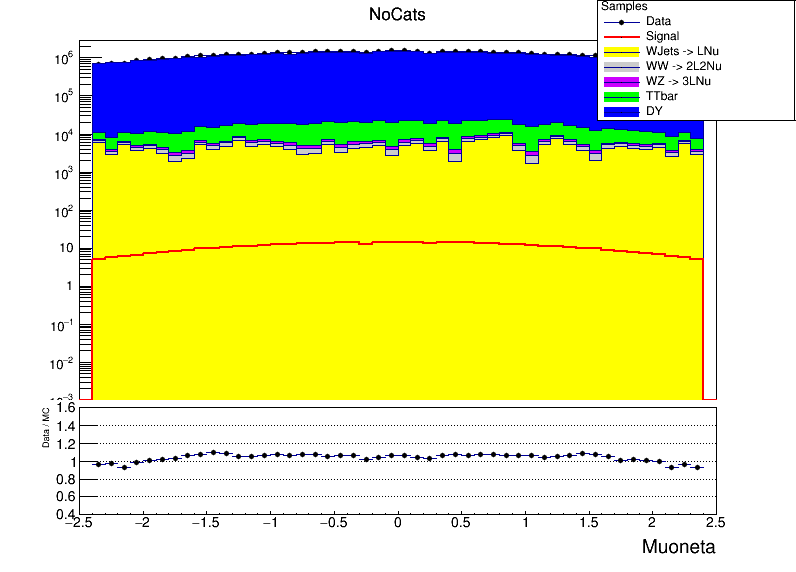
\includegraphics[width=0.45\linewidth]{figures/ch_higgs/distributions/baseline_kalman/distribution__NoCats__Muoneta__logY.png}\\
    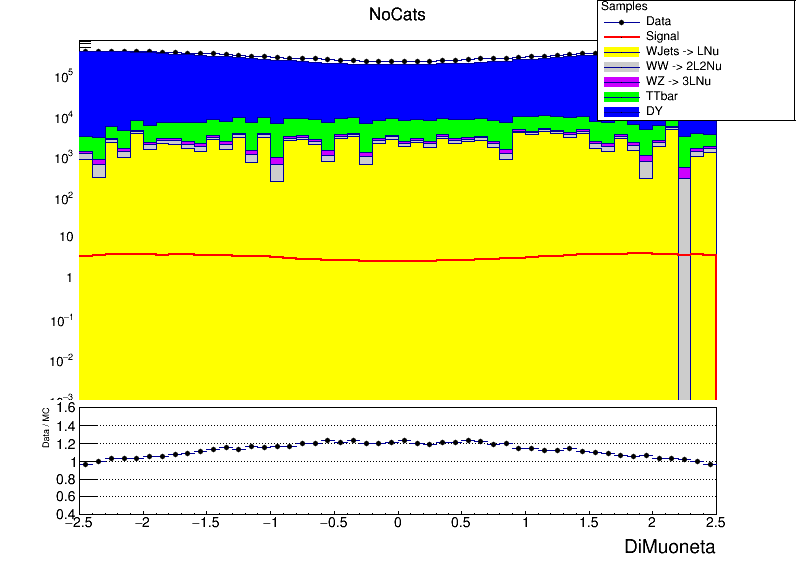
\includegraphics[width=0.45\linewidth]{figures/ch_higgs/distributions/baseline_kalman/distribution__NoCats__DiMuoneta__logY.png}
    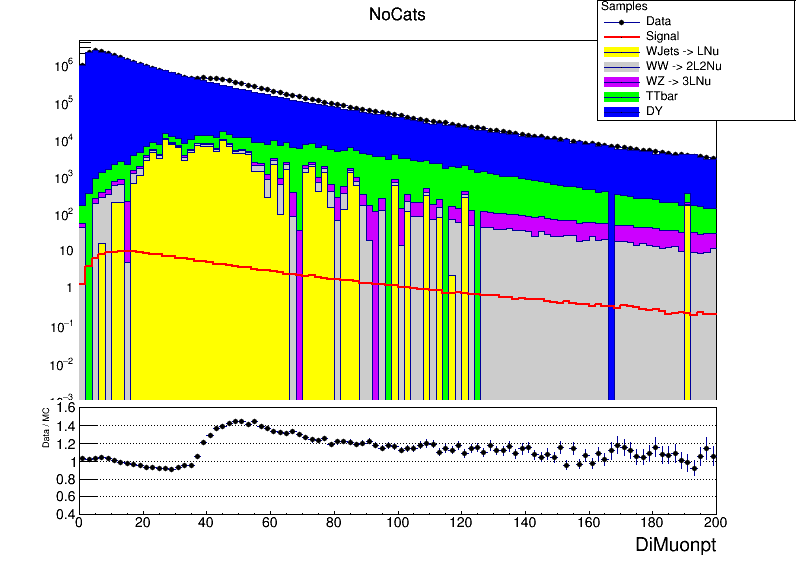
\includegraphics[width=0.45\linewidth]{figures/ch_higgs/distributions/baseline_kalman/distribution__NoCats__DiMuonpt__logY.png}
    \caption{Inclusive Kinematic Distributions: muon p$_t$ (top left), muon $\eta$ (top right), dimuon $\eta$ (bottom left) and dimuon p$_t$ (bottom right). Discrepancy between data and simulated backgrounds is observed for muon p$_t$ and dimuon p$_t$.}
    \label{fig:higgs_selections_inclusivekinematic}
  \end{figure}
% \begin{figure}[htbp]
%    \centering
%    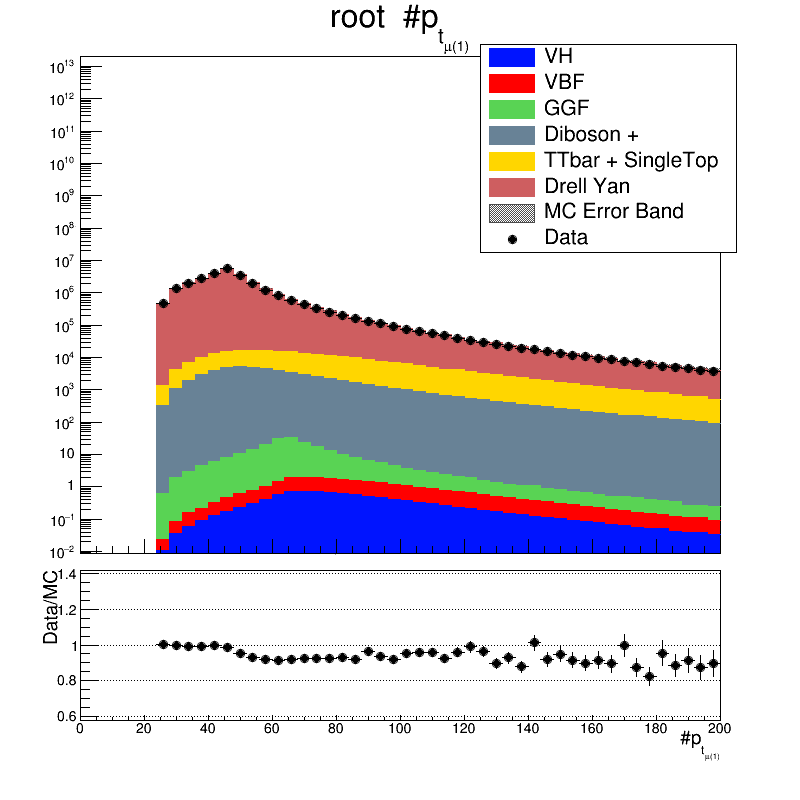
\includegraphics[width=0.45\textwidth]{figures/event_sel/mu1_pt_root.png}
%    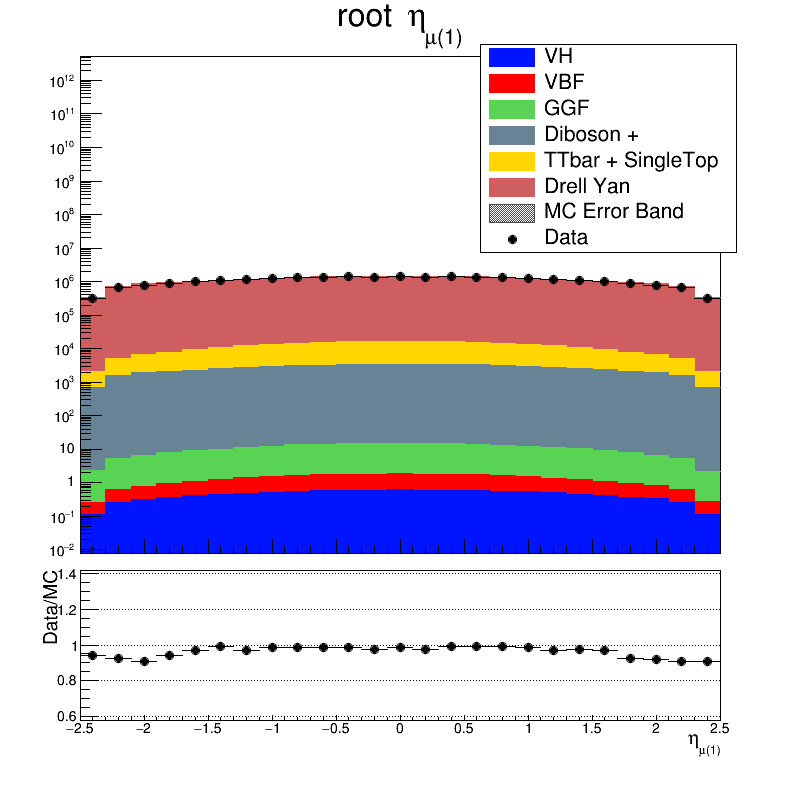
\includegraphics[width=0.45\textwidth]{figures/event_sel/mu1_eta_root.png}\\
%    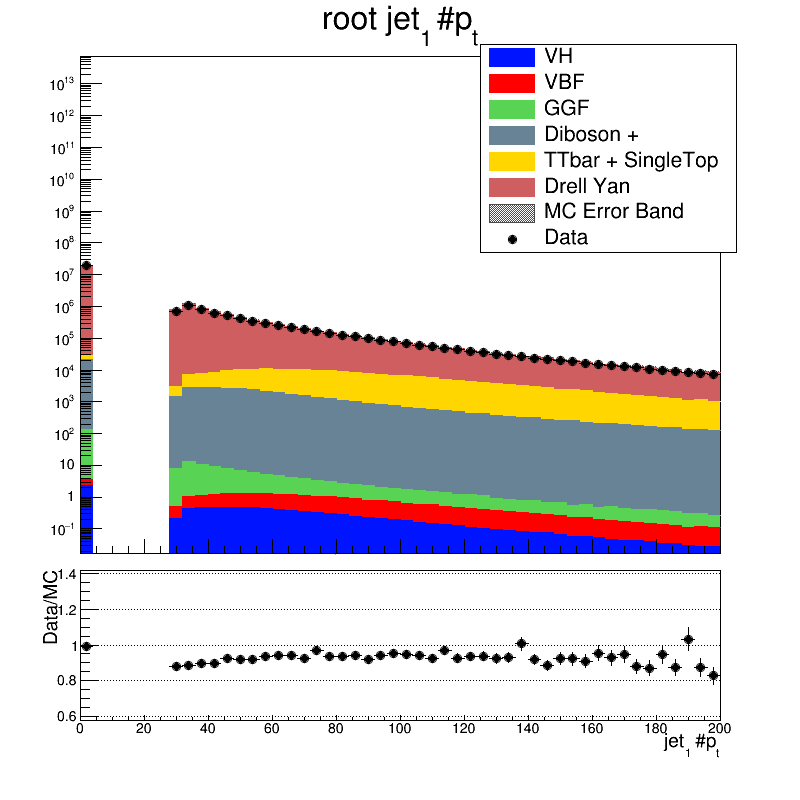
\includegraphics[width=0.45\textwidth]{figures/event_sel/jet1_pt_root.png}
%    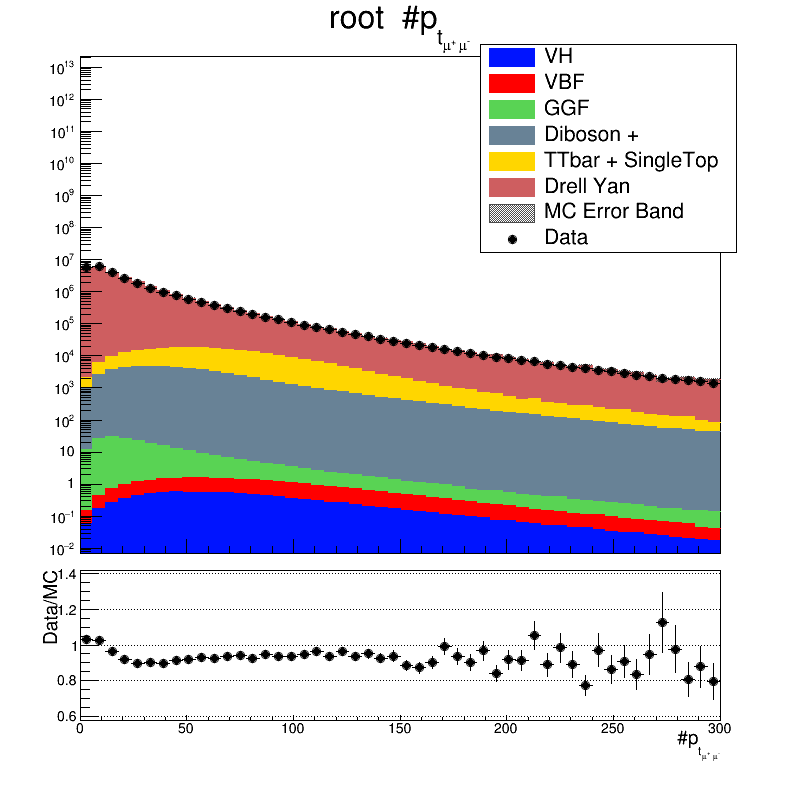
\includegraphics[width=0.45\textwidth]{figures/event_sel/dimu_pt_root.png}
%    \caption{Inclusive Kinematic Distributions}
%    \label{fig:higgs_selections_inclusivekinematic}
%  \end{figure}

Furthermore, in Figure~\ref{fig:higgs_selections_inclusivemass}, the inclusive dimuon mass distributions are shown with Rochester and Kalman corrections respectively applied to both Data and Monte Carlo. Notice that the discrepancy in scale and resolution is no longer present around the Z mass ($\approx 91$ GeV) peak. Overall, comparing collision data with the simulated backgrounds, the dimuon mass distribution is well modeled.
\begin{figure}[htbp]
  \centering
  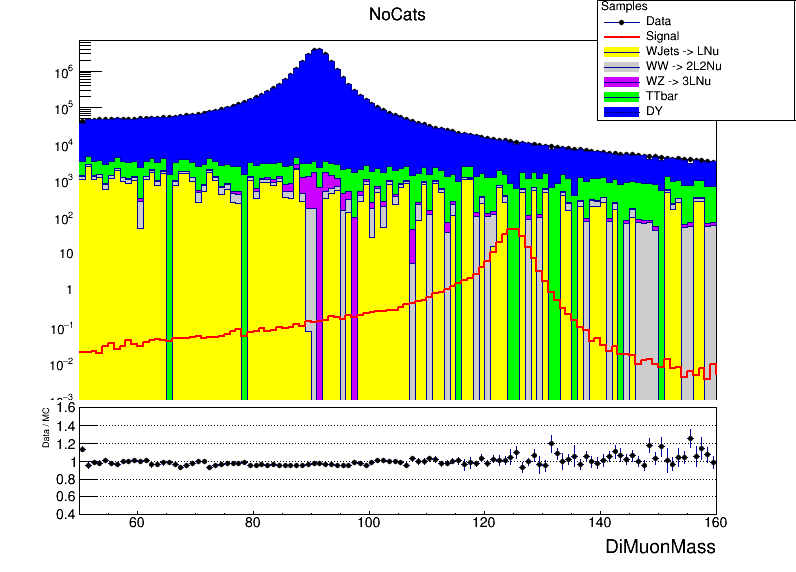
\includegraphics[width=0.9\linewidth]{figures/ch_higgs/distributions/baseline_rochester/distribution__NoCats__DiMuonMass__logY.png}\\
  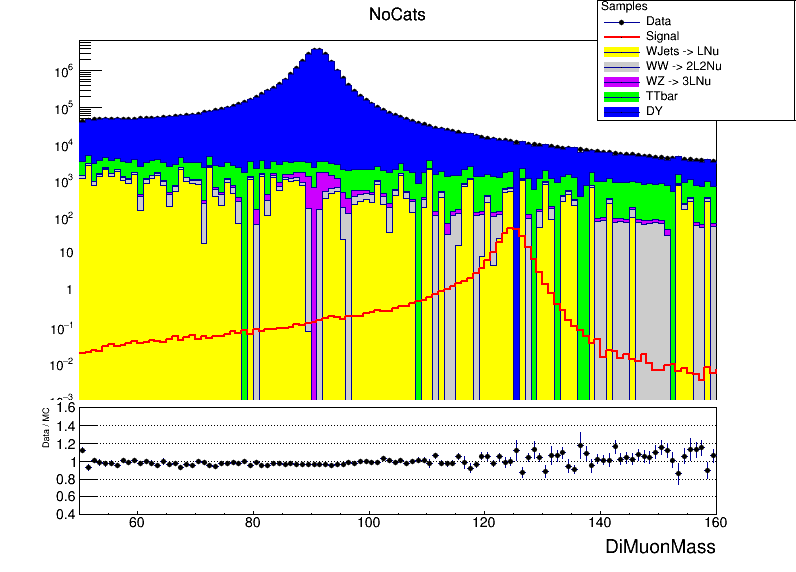
\includegraphics[width=0.9\linewidth]{figures/ch_higgs/distributions/baseline_kalman/distribution__NoCats__DiMuonMass__logY.png}
  \caption{Inclusive Dimuon Mass Distributions. Rochester (Left) and Kalman (Right) Corrections applied. Comparison of data (black points) and simulated backgrounds (stacked). 125 GeV Higgs Boson signal is shown as a red solid line.}
  \label{fig:higgs_selections_inclusivemass}
\end{figure}



% \subsection{Object validation}
% After applying all the selection cuts and scale factors, we validate the MC simulation
% on data events where the candidate muon pair has an invariant mass greater than 60~GeV.

% \begin{figure}[hbp]
%   \centering
%   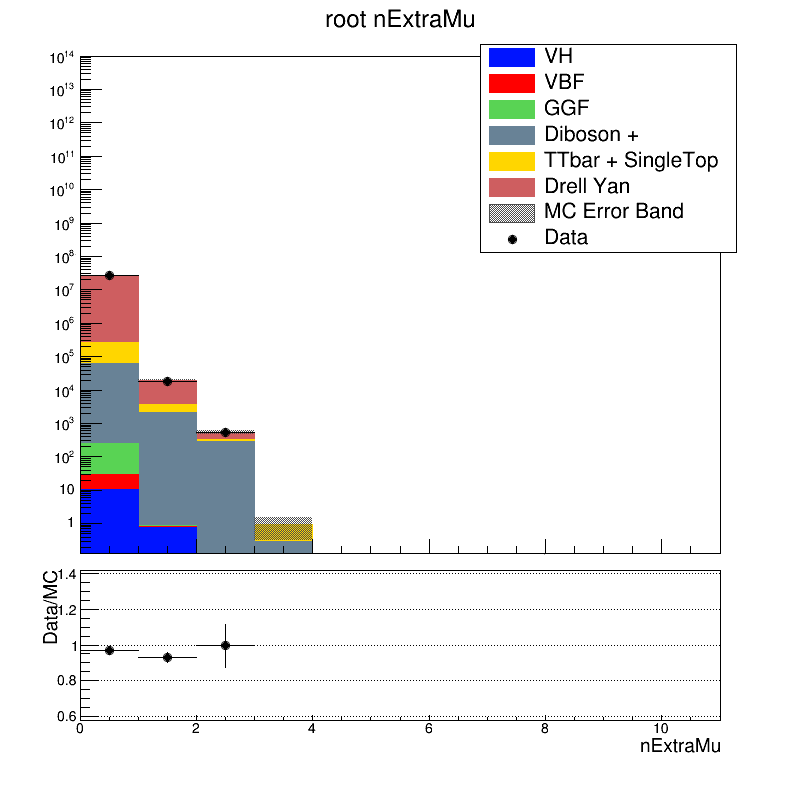
\includegraphics[width=0.32\linewidth]{figures/event_sel/nExtraMu_root.png}
%   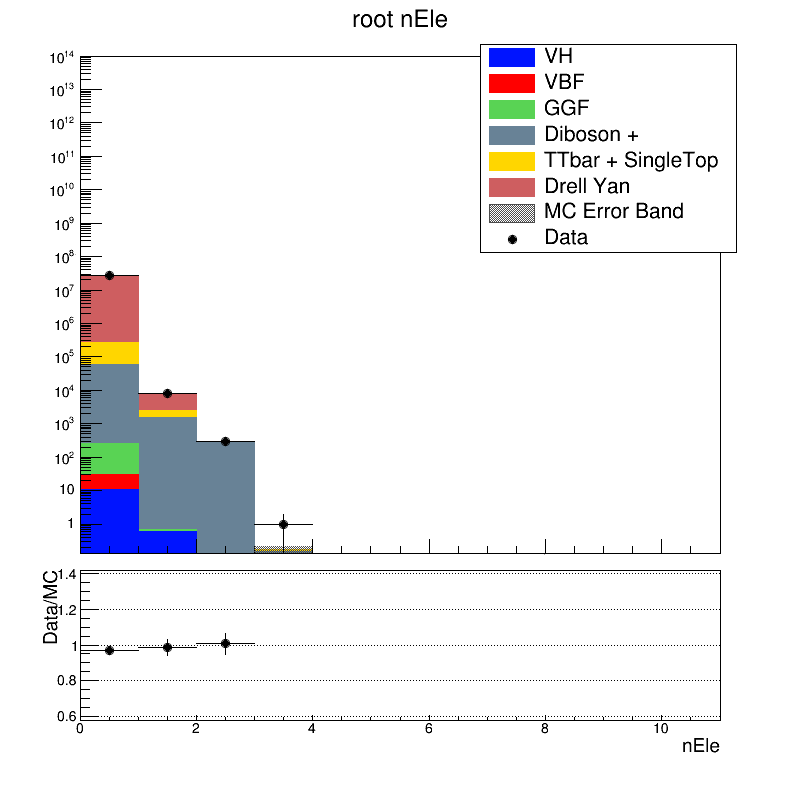
\includegraphics[width=0.32\linewidth]{figures/event_sel/nEle_root.png}
%   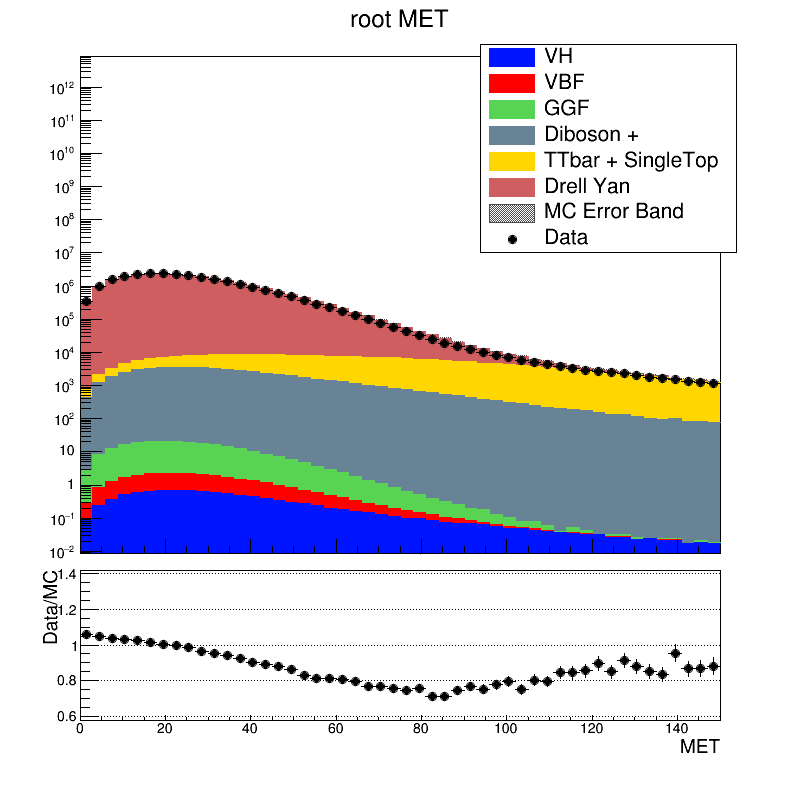
\includegraphics[width=0.32\linewidth]{figures/event_sel/MET_root.png}
%   \caption
%    {Validation of global event variables.}
%   \label{fig:valid_evt}
% \end{figure}

% \begin{figure}[hbp]
%   \centering
%   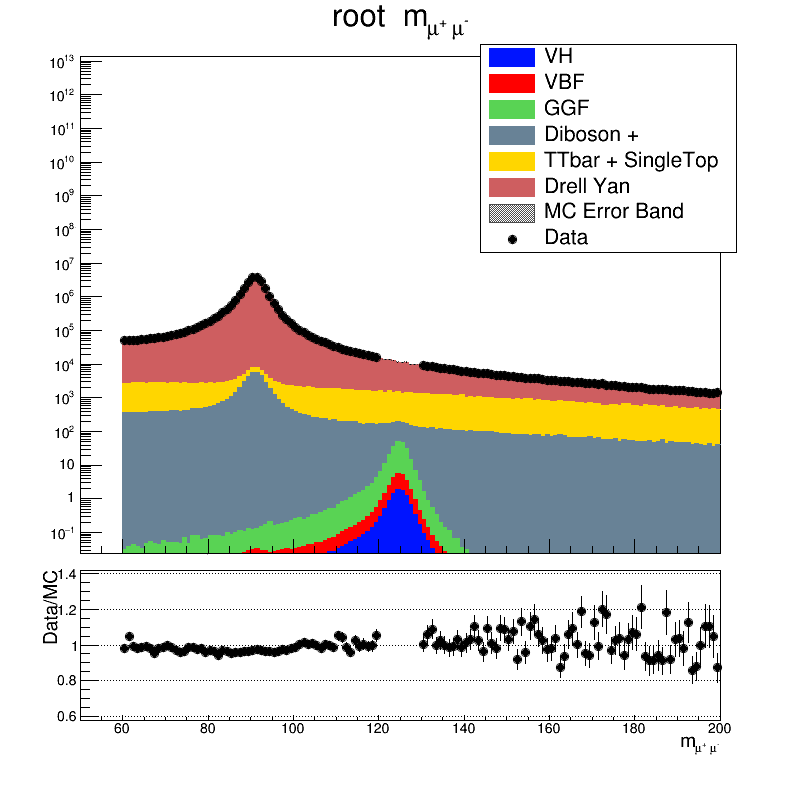
\includegraphics[width=0.32\linewidth]{figures/event_sel/dimu_mass_Roch_root.png}
%   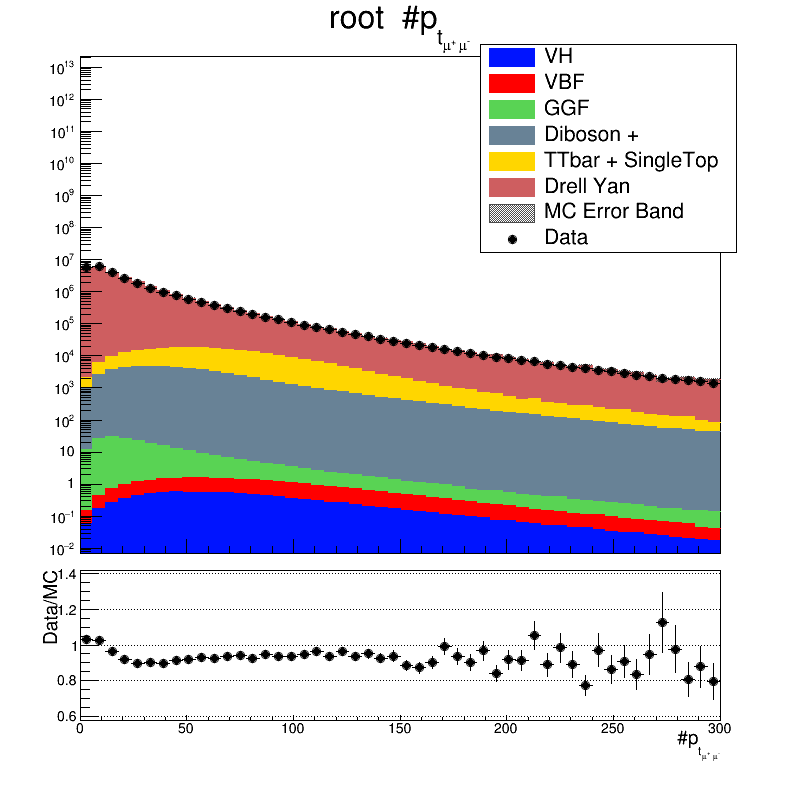
\includegraphics[width=0.32\linewidth]{figures/event_sel/dimu_pt_root.png}
%   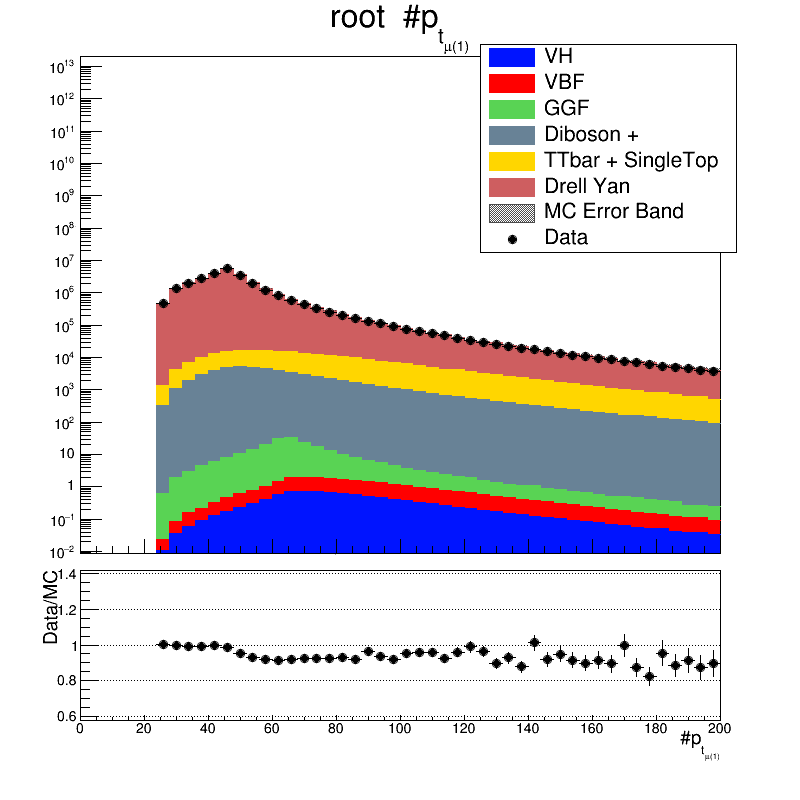
\includegraphics[width=0.32\linewidth]{figures/event_sel/mu1_pt_root.png}
%   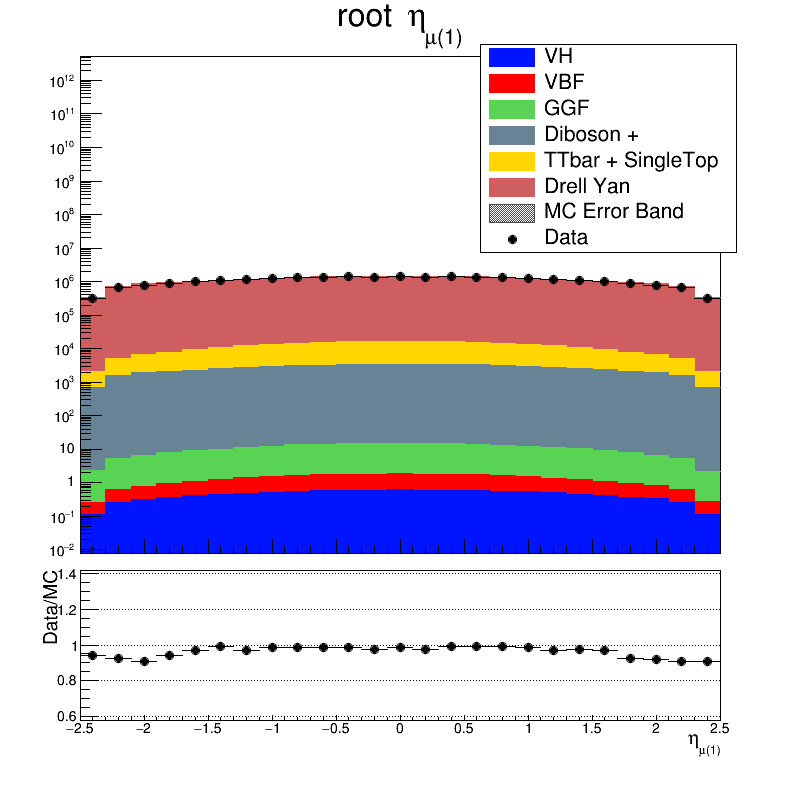
\includegraphics[width=0.32\linewidth]{figures/event_sel/mu1_eta_root.png}
%   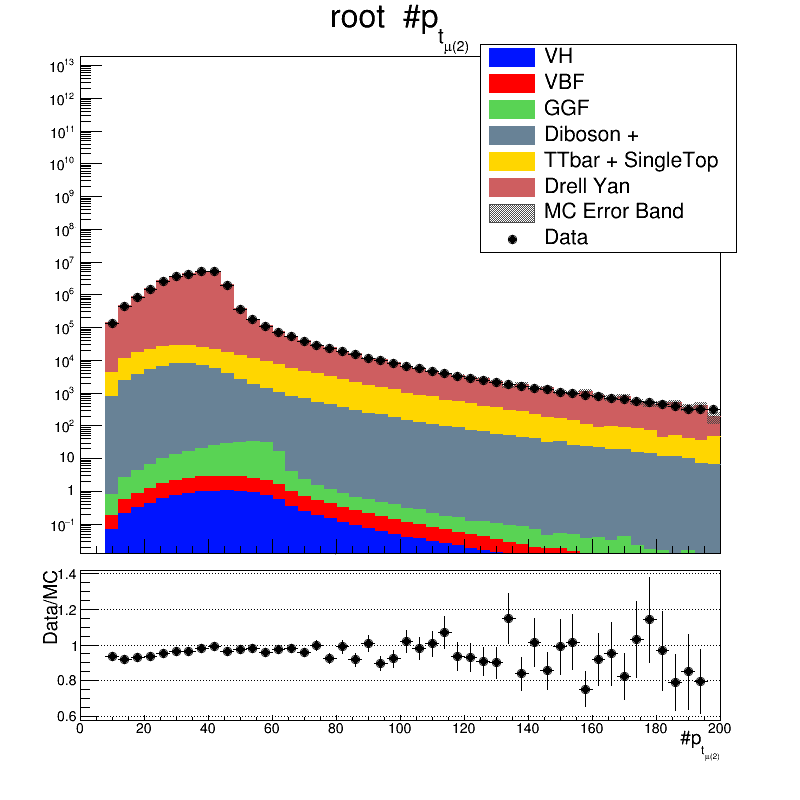
\includegraphics[width=0.32\linewidth]{figures/event_sel/mu2_pt_root.png}
%   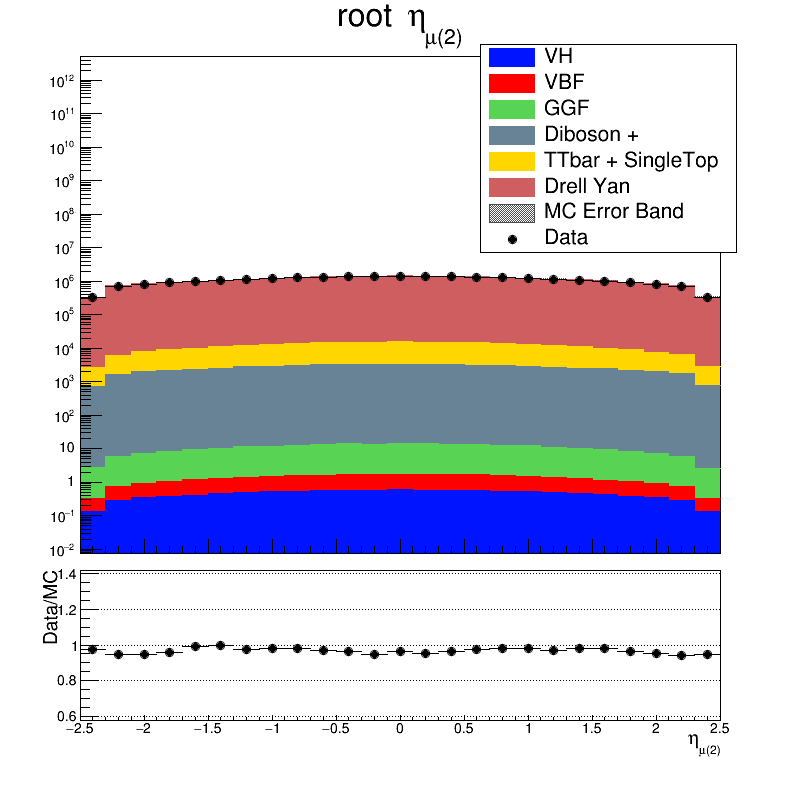
\includegraphics[width=0.32\linewidth]{figures/event_sel/mu2_eta_root.png}
%   \caption
%    {Validation of muon-related variables.}
%   \label{fig:valid_muons}
% \end{figure}

% \begin{figure}[hbp]
%   \centering
%   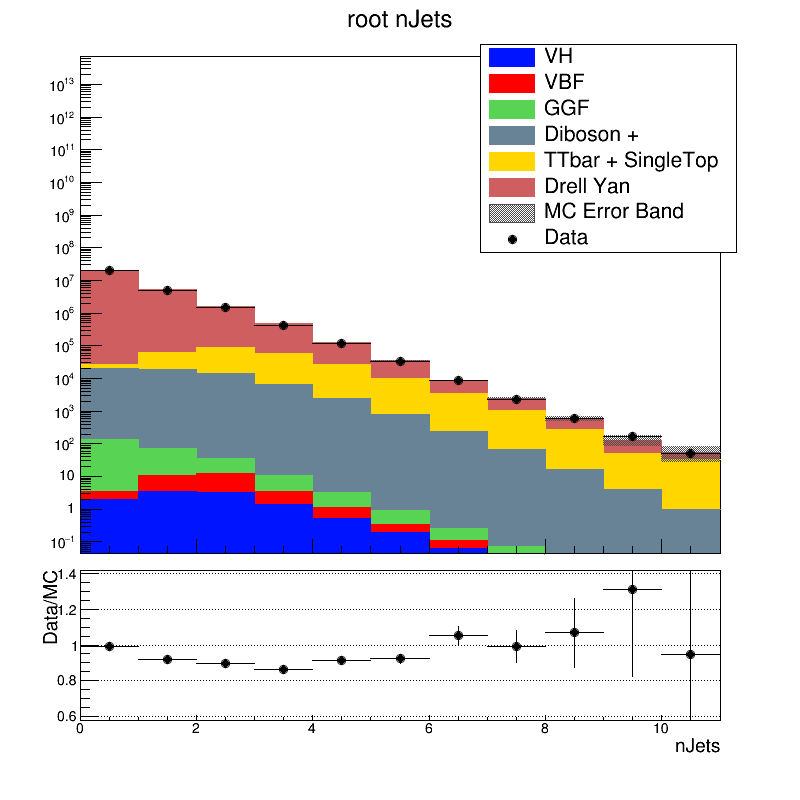
\includegraphics[width=0.32\linewidth]{figures/event_sel/nJets_root.png}
%   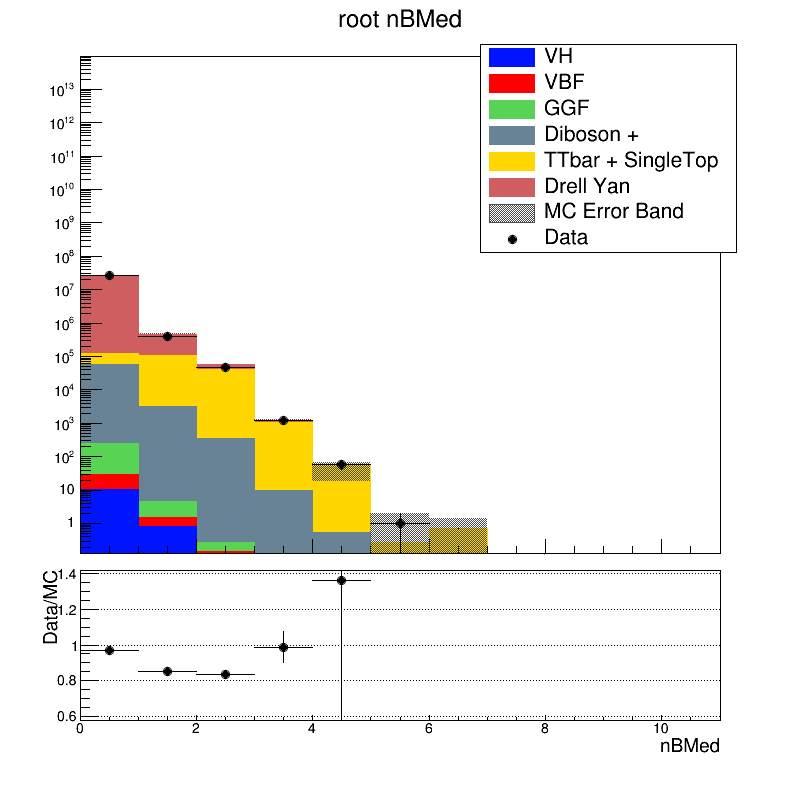
\includegraphics[width=0.32\linewidth]{figures/event_sel/nBMed_root.png}
%   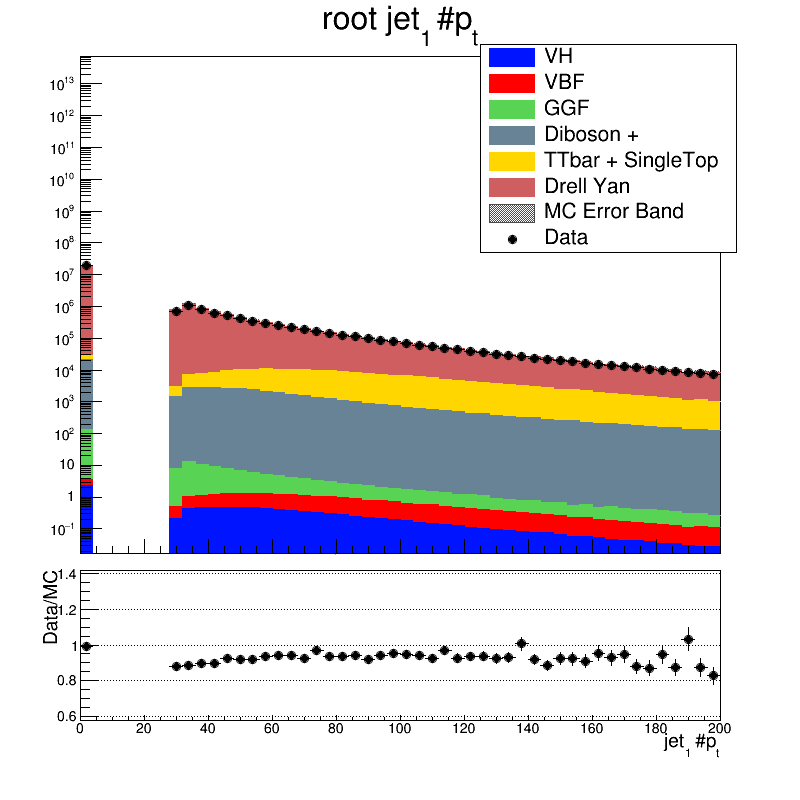
\includegraphics[width=0.32\linewidth]{figures/event_sel/jet1_pt_root.png}
%   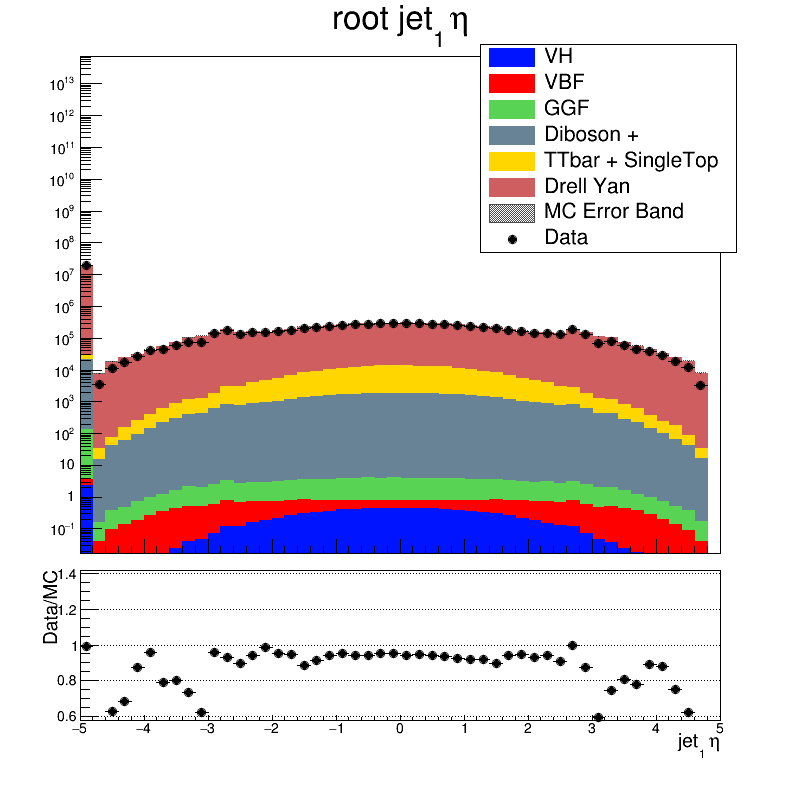
\includegraphics[width=0.32\linewidth]{figures/event_sel/jet1_eta_root.png}
%   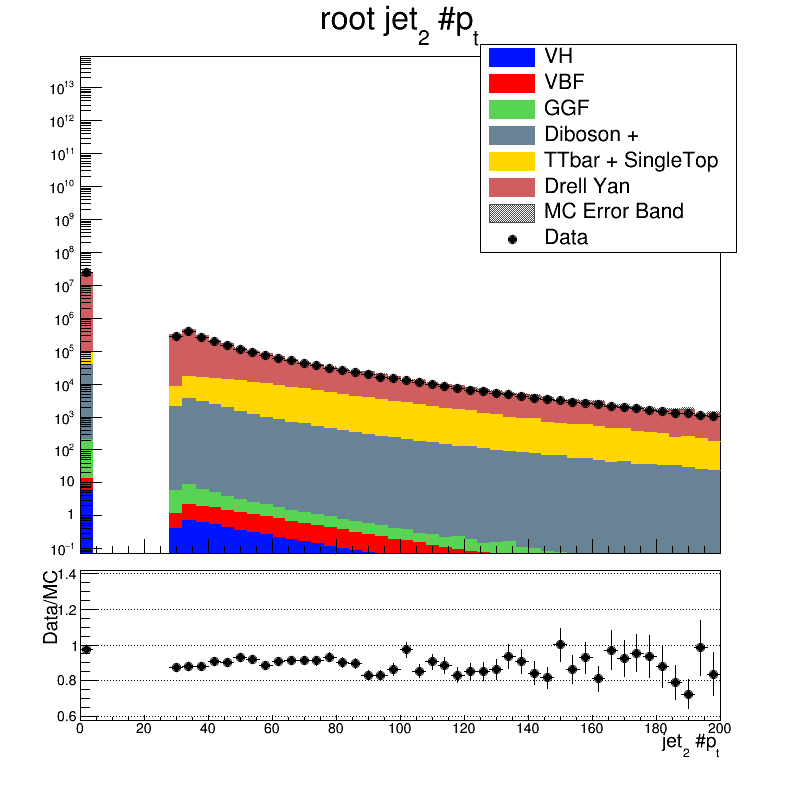
\includegraphics[width=0.32\linewidth]{figures/event_sel/jet2_pt_root.png}
%   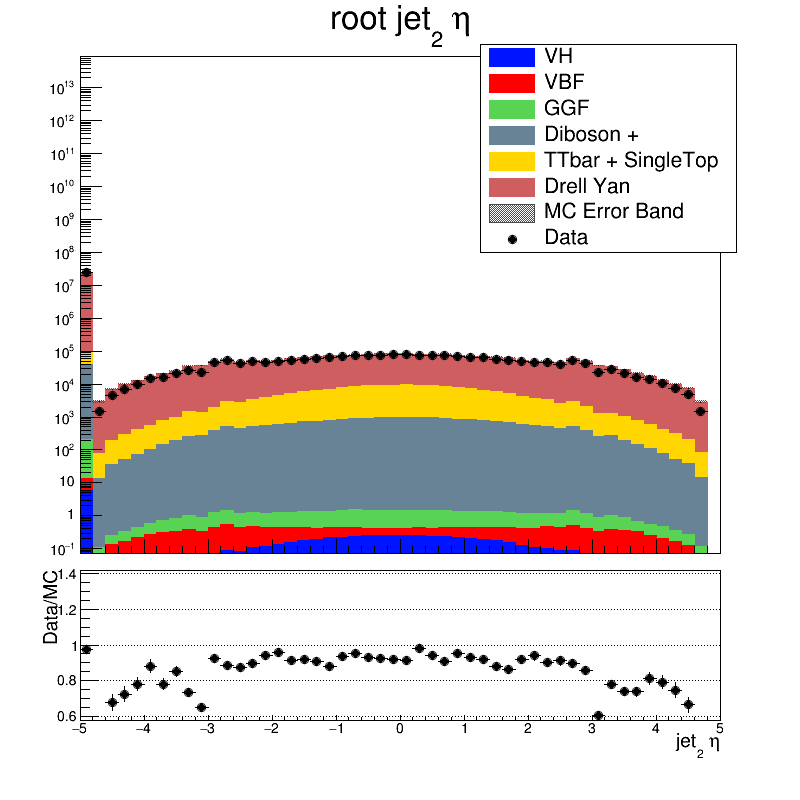
\includegraphics[width=0.32\linewidth]{figures/event_sel/jet2_eta_root.png}
%   \caption
%    {Validation of jet-related variables.}
%   \label{fig:valid_jets}
% \end{figure}



